\documentclass{article}
\title{Exponential function}
\author{Michael Iversen}
\usepackage{graphicx}
\begin{document}
\maketitle
The exponential function is denoted either by $\exp(x)$ or $e^x$. It is defined by the following power series
\begin{equation}
\exp(x) = \sum_{n=0}^\infty \frac{x^n}{n!}.
\end{equation}
The exponential function has several properties worth noting. First, it satisfies the exponentiation identity
\begin{equation}
\exp(x + y) = \exp(x) \cdot \exp(y).
\end{equation}
Secondly, it is its own derivative,
\begin{equation}
\frac{\mathrm d}{\mathrm dx} \exp(x) = \exp(x).
\end{equation}
When implementing the exponential function numerically, it is efficient to use the following expression
\begin{equation}\label{eq:expression}
\exp(x) = 1 + x \cdot \left( 1 + \frac{x}{2} \left( 1 + \frac{x}{3} \left ( 1 + \ldots \right)\right)\right).
\end{equation}
One may check that the right hand side of the above equation is equivalent to the power series by expanding the expression.
In the implementation, we only include terms up to order $x^{10}$. 
We also demand that if $x \leq 0$ then the function calls itself with argument $-x$, i.e. $1 / \exp(-x)$.
Mathematically, these two expressions are of course identical $1 / \exp(-x) = \exp(x)$ but numerically it makes a big difference.
The expression in equation (\ref{eq:expression}) (including only terms up to order $x^{10}$) is only a good approximation for $x$ close to zero.
While the approximation is inaccurate at large netaive $x$, the condition $\exp(x) \to 1/\exp(-x)$ for negative $x$ ensures the correct behaviour for $x < 0$.
Furthermore, in the implementation, we demand that when $x > 1/8$ we call the function itself with a smaller input $\exp(x/2)^2$.
Again, this detail improves performance because $\exp(x/2)$ is more accurate since $x/2$ is smaller than $x$.
We can check numerically that the implementation works by plotting it along with precalculated values. 
This plot can be seen in figure \ref{fig:exp}.
\begin{figure}
\centering
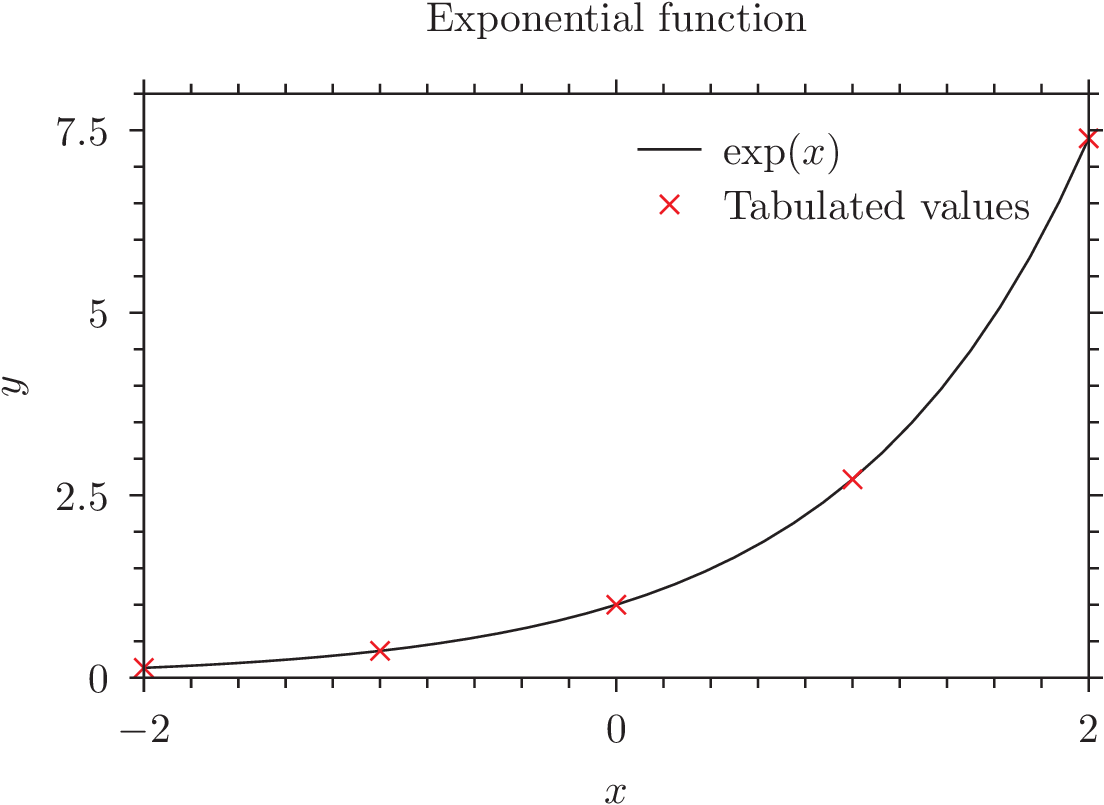
\includegraphics{ex.png}
\caption{The exponential function calculated from equation (\ref{eq:expression}) and tabular values.}
\label{fig:exp}
\end{figure}
It is clear from the figure that the expression correctly computes the exponential function. 

\end{document}
